\documentclass[10pt, a4paper]{amsart}

\usepackage[]{graphicx}
\usepackage[]{hyperref}
\usepackage[]{physics}
\usepackage[]{listings}
\usepackage[T1]{fontenc}
\usepackage{subfig}
\usepackage{color}
\definecolor{gray}{rgb}{0.5,0.5,0.5}

\lstset{ %
  backgroundcolor=\color{white}, 
  basicstyle=\footnotesize,      
  breakatwhitespace=false,       
  breaklines=true,               
  captionpos=b,                  
  commentstyle=\color{green},    
  frame=single,	                 
  keepspaces=true,               
  keywordstyle=\color{blue},     
  language=fortran ,             
  rulecolor=\color{black},       
  showspaces=false,              
  showstringspaces=false,        
  showtabs=false,                
  stepnumber=2,                  
  stringstyle=\color{mauve},   
  tabsize=2,	                 
}

\title{Project 1 - Tridiagonal Matrix Solver}

\author{Marco Santia}

\begin{document}
\begin{abstract}
Numerical methods for discretizing linear second-order differential equations are compared for the one-dimensional Poisson equation case. Finite-difference discretization in this case produces a tridiagonal matrix when using Dirichlet boundary conditions that is solved with a simplified Gauss-elimination algorithm know as the Thomas algorithm. The problem is then solved using a problem-specific variant of the Thomas algorithm as well as a LU-decomposition method requiring full matrix-construction. It was found that all three methods produce very high accuracy with respect to the exact solution for moderately sized grids. The LU decomposition method becomes memory restrictive without sparse matrix methods for large grid sizes. We find the problem specific algorithm to provide relative speedups compared to the general Thomas algorithm. Both of which scale linearly with grid size compared to the cubic scaling of the LU method. 

\end{abstract}
\maketitle
\section{Introduction}
Many physical phenomena can be described by elliptical partial differential equations which contain second order derivatives. For example in semiconductor device modeling the charge density $\rho$ the Poisson equation is used
\begin{equation}
\nabla^2 \Phi = \frac{q}{e}(n-p+N_A-N_D)
\end{equation}
For these devices it is essential to determine population densities of acceptors $N_A$ and donors $N_D$ as well as electrons $n$ and holes $p$. In this work, a simplified model of the more general equation is solved using a spherically symmetric system in one dimension:
\begin{equation}
\frac{d^2\phi}{dr^2}=-4\pi r\rho(r)
\end{equation}
and by letting $\phi \rightarrow u$ and $r \rightarrow x$ we get
\begin{equation}
-u''(x)=f(x) 
\end{equation}
For the purpose of this work we utilize Dirichlet boundary conditions for simplicity and a source function $f(x) = 100e^{-10x}$ with a known analytical solution $u(x) = 1-(1-e^{-10})x-e^{-10x}$ to compare to. This allows for the system to be rewritten by a set of linear equations. The solution variables are written as $v_i$ with grid points $x_i=ih$ and a grid spacing of $h=\frac{1}{n+1}$ from $x_0 = 0$ to $x_{n+1}=1$. The dirichlet boundary conditions are expressed as $v_0=v_n+1=0$ which leads to the approximation:
\begin{equation}
-\frac{v_{i+1}-2v_i+v_{i-1}}{h^2}=f_i 
\end{equation}
by then rearranging this equation and defining $\tilde{b}_i=h^2 f_i$ we get
\begin{equation}
-v_{i+1}-2v_i+v_{i-1}=\tilde{b}_i
\end{equation}
which can be written in matrix form 
\begin{equation*}
   \mathbf{A}\mathbf{v} = \tilde{\mathbf{b}},
\end{equation*}
where $\mathbf{A}$ is an $n\times n$  tridiagonal matrix which we rewrite as

\[
    \mathbf{A} = \begin{bmatrix}
                           2& -1& 0 &\dots   & \dots &0 \\
                           -1 & 2 & -1 &0 &\dots &\dots \\
                           0&-1 &2 & -1 & 0 & \dots \\
                           & \dots   & \dots &\dots   &\dots & \dots \\
                           0&\dots   &  &-1 &2& -1 \\
                           0&\dots    &  & 0  &-1 & 2 \\
                      \end{bmatrix},
\]I

\section{General Thomas Algorithm}
For a general matrix that does not necessarily have the tridiagonal property, the linear system could be solved by Gaussian elimination. Although effective, the method scales as $\frac{1}{3}(n^3+3n^2-n)$ which is extremely inefficient when considering the desirable matrix properties our system contains. In addition to repeated values down the diagonals, we have a high degree of sparsity and tridiagonal structure. As with many sparse matrices, it would be ideal to construct an iterative approach that does not require explicit matrix construction and avoids any gaussian elimination steps that are trivial. To remedy this, we utilize the Thomas algorithm \cite{recipes}. To begin in a more general framework, we do not assume the diagonals of our matrix contain only one repeated value. The steps are summarized:

\begin{align}
m &= \frac{a_k}{b_{k-1}}\\ 
b_k &= b_k-mc_{k-1}\\ 
\tilde{b}_k &= \tilde{b}_k-m\tilde{b}_{k-1}
\end{align}

and equivalently in FORTRAN code,
\lstinputlisting[language=fortran, firstline=6, lastline=26]{linalg.f90}

repeating these operators will triangularize the matrix such that the solution can be computed through a simple backwards substitution:
\begin{equation}
v_n = \frac{\tilde{b}_n}{b_n}
\end{equation}
iterating in reverse from $k = n-1$ to $k = 1$,
\begin{equation}
v_k = \frac{\tilde{b}_k-c_k v_{k+1}}{b_k} 
\end{equation}

The backward substitution is implemented in FORTRAN like so:
\lstinputlisting[language=fortran, firstline=28,lastline=32]{linalg.f90}

This method will be much more efficient as it does not require matrix computations over the sparse majority of the matrix. In terms of floating point operations, there will be 6 FLOPS per iteration in the forward substitution and additional 2 from the backward substitution. This gives a total of $8(N-1)$ flops which is approximately $O(N)$.

\section{Specialized Thomas Algorithm}
For the specific matrix used in this case, we can use the property that the diagonals contain the same value for all $i$ to precompute values when possible and further speed up the algorithm as shown in the following code:

\lstinputlisting[language=fortran, firstline=50,lastline=61]{linalg.f90}

\section{LU Decomposition}
In the general case of a system $A\vec{v}=\vec{f}$, we can solve the system for any non-singular, invertible matrix $A$ using the LU decomposition method. This consists of rewriting the system as a matrix product between the lower and upper triangular constituents (L and U respectively) i.e $A=LU$. This decomposition consists of determining
\begin{equation}
L =
\begin{bmatrix}
1 & 0 & 0 & \dots & 0 & 0 \\
l_{21} & 1 & 0 & \dots & 0 & 0 \\
l_{31} & l_{32} & 1 & \dots & 0 & 0 \\
  &\vdots & & \ddots & \vdots  & \\
l_{n-11} & l_{n-12} & l_{n-13} & \dots & 1 & 0 \\  
l_{n1} & l_{n2} & l_{n3} & \dots & l_{nn-1} & 1
\end{bmatrix}
\end{equation}

as well as 
\begin{equation}
U = 
\begin{bmatrix}
u_{11} & u_{12} & u_{13} & \dots & u_{1n-1} & u_{1n} \\
0 & u_{22} & u_{23} & \dots & u_{2n-1} & u_{2n} \\
0 & 0 & u_{33} & \dots & u_{3n-1} & u_{3n} \\
  &\vdots & & \ddots & \vdots  & \\
0 & 0 & 0 & \dots & u_{n-1n-1} & u_{n-1n} \\  
0 & 0 & 0 & \dots & 0 & u_{nn}
\end{bmatrix}
\end{equation}

From here the problem is solved by first computing $L\vec{z}=\vec{f}$ using standard methods and then substituting those results into $U\vec{v}=\vec{z}$. Because this method ultimately reduces the problem to a form where Gaussian elimination becomes usable, the scaling should by on the same order as gaussian elimination $N^3$. 

\section{Results}


\subsection{Convergence}
Comparing to an exact solution for our problem, all algorithms used were found to be sufficiently accurate with a rapidly converging solution with respect to grid size as is shown in \ref{fig:n10} with a grid of $N=100$ being almost exact. The max error with respect to grid size is shown in \ref{fig:error} where we can see the spacing size where machine precision becomes a computational bottleneck.


\begin{figure}%
    \centering
    \subfloat[N=10]{\resizebox{0.45\textwidth}{!}{% GNUPLOT: LaTeX picture with Postscript
\begingroup
  \makeatletter
  \providecommand\color[2][]{%
    \GenericError{(gnuplot) \space\space\space\@spaces}{%
      Package color not loaded in conjunction with
      terminal option `colourtext'%
    }{See the gnuplot documentation for explanation.%
    }{Either use 'blacktext' in gnuplot or load the package
      color.sty in LaTeX.}%
    \renewcommand\color[2][]{}%
  }%
  \providecommand\includegraphics[2][]{%
    \GenericError{(gnuplot) \space\space\space\@spaces}{%
      Package graphicx or graphics not loaded%
    }{See the gnuplot documentation for explanation.%
    }{The gnuplot epslatex terminal needs graphicx.sty or graphics.sty.}%
    \renewcommand\includegraphics[2][]{}%
  }%
  \providecommand\rotatebox[2]{#2}%
  \@ifundefined{ifGPcolor}{%
    \newif\ifGPcolor
    \GPcolortrue
  }{}%
  \@ifundefined{ifGPblacktext}{%
    \newif\ifGPblacktext
    \GPblacktexttrue
  }{}%
  % define a \g@addto@macro without @ in the name:
  \let\gplgaddtomacro\g@addto@macro
  % define empty templates for all commands taking text:
  \gdef\gplbacktext{}%
  \gdef\gplfronttext{}%
  \makeatother
  \ifGPblacktext
    % no textcolor at all
    \def\colorrgb#1{}%
    \def\colorgray#1{}%
  \else
    % gray or color?
    \ifGPcolor
      \def\colorrgb#1{\color[rgb]{#1}}%
      \def\colorgray#1{\color[gray]{#1}}%
      \expandafter\def\csname LTw\endcsname{\color{white}}%
      \expandafter\def\csname LTb\endcsname{\color{black}}%
      \expandafter\def\csname LTa\endcsname{\color{black}}%
      \expandafter\def\csname LT0\endcsname{\color[rgb]{1,0,0}}%
      \expandafter\def\csname LT1\endcsname{\color[rgb]{0,1,0}}%
      \expandafter\def\csname LT2\endcsname{\color[rgb]{0,0,1}}%
      \expandafter\def\csname LT3\endcsname{\color[rgb]{1,0,1}}%
      \expandafter\def\csname LT4\endcsname{\color[rgb]{0,1,1}}%
      \expandafter\def\csname LT5\endcsname{\color[rgb]{1,1,0}}%
      \expandafter\def\csname LT6\endcsname{\color[rgb]{0,0,0}}%
      \expandafter\def\csname LT7\endcsname{\color[rgb]{1,0.3,0}}%
      \expandafter\def\csname LT8\endcsname{\color[rgb]{0.5,0.5,0.5}}%
    \else
      % gray
      \def\colorrgb#1{\color{black}}%
      \def\colorgray#1{\color[gray]{#1}}%
      \expandafter\def\csname LTw\endcsname{\color{white}}%
      \expandafter\def\csname LTb\endcsname{\color{black}}%
      \expandafter\def\csname LTa\endcsname{\color{black}}%
      \expandafter\def\csname LT0\endcsname{\color{black}}%
      \expandafter\def\csname LT1\endcsname{\color{black}}%
      \expandafter\def\csname LT2\endcsname{\color{black}}%
      \expandafter\def\csname LT3\endcsname{\color{black}}%
      \expandafter\def\csname LT4\endcsname{\color{black}}%
      \expandafter\def\csname LT5\endcsname{\color{black}}%
      \expandafter\def\csname LT6\endcsname{\color{black}}%
      \expandafter\def\csname LT7\endcsname{\color{black}}%
      \expandafter\def\csname LT8\endcsname{\color{black}}%
    \fi
  \fi
    \setlength{\unitlength}{0.0500bp}%
    \ifx\gptboxheight\undefined%
      \newlength{\gptboxheight}%
      \newlength{\gptboxwidth}%
      \newsavebox{\gptboxtext}%
    \fi%
    \setlength{\fboxrule}{0.5pt}%
    \setlength{\fboxsep}{1pt}%
\begin{picture}(7200.00,5040.00)%
    \gplgaddtomacro\gplbacktext{%
      \csname LTb\endcsname%
      \put(814,704){\makebox(0,0)[r]{\strut{}$0$}}%
      \put(814,1286){\makebox(0,0)[r]{\strut{}$0.1$}}%
      \put(814,1867){\makebox(0,0)[r]{\strut{}$0.2$}}%
      \put(814,2449){\makebox(0,0)[r]{\strut{}$0.3$}}%
      \put(814,3030){\makebox(0,0)[r]{\strut{}$0.4$}}%
      \put(814,3612){\makebox(0,0)[r]{\strut{}$0.5$}}%
      \put(814,4193){\makebox(0,0)[r]{\strut{}$0.6$}}%
      \put(814,4775){\makebox(0,0)[r]{\strut{}$0.7$}}%
      \put(946,484){\makebox(0,0){\strut{}$0$}}%
      \put(1532,484){\makebox(0,0){\strut{}$0.1$}}%
      \put(2117,484){\makebox(0,0){\strut{}$0.2$}}%
      \put(2703,484){\makebox(0,0){\strut{}$0.3$}}%
      \put(3289,484){\makebox(0,0){\strut{}$0.4$}}%
      \put(3875,484){\makebox(0,0){\strut{}$0.5$}}%
      \put(4460,484){\makebox(0,0){\strut{}$0.6$}}%
      \put(5046,484){\makebox(0,0){\strut{}$0.7$}}%
      \put(5632,484){\makebox(0,0){\strut{}$0.8$}}%
      \put(6217,484){\makebox(0,0){\strut{}$0.9$}}%
      \put(6803,484){\makebox(0,0){\strut{}$1$}}%
    }%
    \gplgaddtomacro\gplfronttext{%
      \csname LTb\endcsname%
      \put(176,2739){\rotatebox{-270}{\makebox(0,0){\strut{}$v_i$}}}%
      \put(3874,154){\makebox(0,0){\strut{}$x_i$}}%
      \csname LTb\endcsname%
      \put(5816,4602){\makebox(0,0)[r]{\strut{}General GaussElim}}%
      \csname LTb\endcsname%
      \put(5816,4382){\makebox(0,0)[r]{\strut{}Exact}}%
      \csname LTb\endcsname%
      \put(5816,4162){\makebox(0,0)[r]{\strut{}LU method}}%
      \csname LTb\endcsname%
      \put(5816,3942){\makebox(0,0)[r]{\strut{}Simple GaussElim}}%
    }%
    \gplbacktext
    \put(0,0){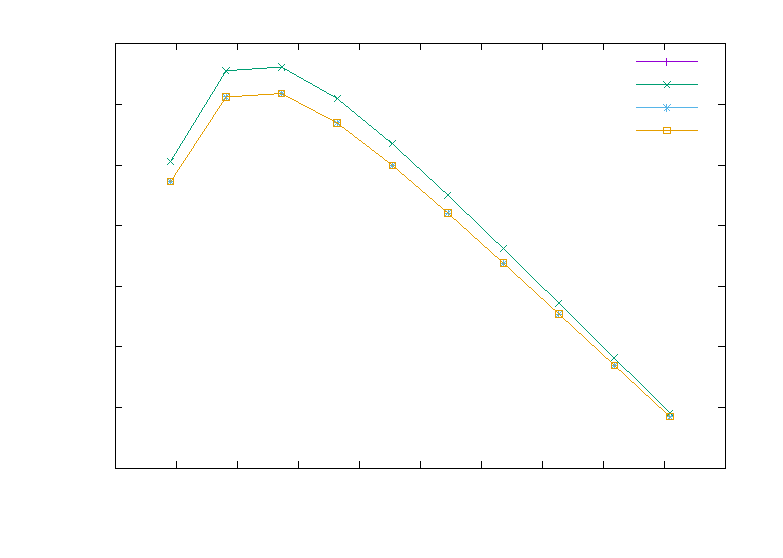
\includegraphics{solutionN10}}%
    \gplfronttext
  \end{picture}%
\endgroup
 }}%
    \qquad
    \subfloat[N=100]{\resizebox{0.45\textwidth}{!}{% GNUPLOT: LaTeX picture with Postscript
\begingroup
  \makeatletter
  \providecommand\color[2][]{%
    \GenericError{(gnuplot) \space\space\space\@spaces}{%
      Package color not loaded in conjunction with
      terminal option `colourtext'%
    }{See the gnuplot documentation for explanation.%
    }{Either use 'blacktext' in gnuplot or load the package
      color.sty in LaTeX.}%
    \renewcommand\color[2][]{}%
  }%
  \providecommand\includegraphics[2][]{%
    \GenericError{(gnuplot) \space\space\space\@spaces}{%
      Package graphicx or graphics not loaded%
    }{See the gnuplot documentation for explanation.%
    }{The gnuplot epslatex terminal needs graphicx.sty or graphics.sty.}%
    \renewcommand\includegraphics[2][]{}%
  }%
  \providecommand\rotatebox[2]{#2}%
  \@ifundefined{ifGPcolor}{%
    \newif\ifGPcolor
    \GPcolortrue
  }{}%
  \@ifundefined{ifGPblacktext}{%
    \newif\ifGPblacktext
    \GPblacktexttrue
  }{}%
  % define a \g@addto@macro without @ in the name:
  \let\gplgaddtomacro\g@addto@macro
  % define empty templates for all commands taking text:
  \gdef\gplbacktext{}%
  \gdef\gplfronttext{}%
  \makeatother
  \ifGPblacktext
    % no textcolor at all
    \def\colorrgb#1{}%
    \def\colorgray#1{}%
  \else
    % gray or color?
    \ifGPcolor
      \def\colorrgb#1{\color[rgb]{#1}}%
      \def\colorgray#1{\color[gray]{#1}}%
      \expandafter\def\csname LTw\endcsname{\color{white}}%
      \expandafter\def\csname LTb\endcsname{\color{black}}%
      \expandafter\def\csname LTa\endcsname{\color{black}}%
      \expandafter\def\csname LT0\endcsname{\color[rgb]{1,0,0}}%
      \expandafter\def\csname LT1\endcsname{\color[rgb]{0,1,0}}%
      \expandafter\def\csname LT2\endcsname{\color[rgb]{0,0,1}}%
      \expandafter\def\csname LT3\endcsname{\color[rgb]{1,0,1}}%
      \expandafter\def\csname LT4\endcsname{\color[rgb]{0,1,1}}%
      \expandafter\def\csname LT5\endcsname{\color[rgb]{1,1,0}}%
      \expandafter\def\csname LT6\endcsname{\color[rgb]{0,0,0}}%
      \expandafter\def\csname LT7\endcsname{\color[rgb]{1,0.3,0}}%
      \expandafter\def\csname LT8\endcsname{\color[rgb]{0.5,0.5,0.5}}%
    \else
      % gray
      \def\colorrgb#1{\color{black}}%
      \def\colorgray#1{\color[gray]{#1}}%
      \expandafter\def\csname LTw\endcsname{\color{white}}%
      \expandafter\def\csname LTb\endcsname{\color{black}}%
      \expandafter\def\csname LTa\endcsname{\color{black}}%
      \expandafter\def\csname LT0\endcsname{\color{black}}%
      \expandafter\def\csname LT1\endcsname{\color{black}}%
      \expandafter\def\csname LT2\endcsname{\color{black}}%
      \expandafter\def\csname LT3\endcsname{\color{black}}%
      \expandafter\def\csname LT4\endcsname{\color{black}}%
      \expandafter\def\csname LT5\endcsname{\color{black}}%
      \expandafter\def\csname LT6\endcsname{\color{black}}%
      \expandafter\def\csname LT7\endcsname{\color{black}}%
      \expandafter\def\csname LT8\endcsname{\color{black}}%
    \fi
  \fi
    \setlength{\unitlength}{0.0500bp}%
    \ifx\gptboxheight\undefined%
      \newlength{\gptboxheight}%
      \newlength{\gptboxwidth}%
      \newsavebox{\gptboxtext}%
    \fi%
    \setlength{\fboxrule}{0.5pt}%
    \setlength{\fboxsep}{1pt}%
\begin{picture}(7200.00,5040.00)%
    \gplgaddtomacro\gplbacktext{%
      \csname LTb\endcsname%
      \put(814,704){\makebox(0,0)[r]{\strut{}$0$}}%
      \put(814,1286){\makebox(0,0)[r]{\strut{}$0.1$}}%
      \put(814,1867){\makebox(0,0)[r]{\strut{}$0.2$}}%
      \put(814,2449){\makebox(0,0)[r]{\strut{}$0.3$}}%
      \put(814,3030){\makebox(0,0)[r]{\strut{}$0.4$}}%
      \put(814,3612){\makebox(0,0)[r]{\strut{}$0.5$}}%
      \put(814,4193){\makebox(0,0)[r]{\strut{}$0.6$}}%
      \put(814,4775){\makebox(0,0)[r]{\strut{}$0.7$}}%
      \put(946,484){\makebox(0,0){\strut{}$0$}}%
      \put(1532,484){\makebox(0,0){\strut{}$0.1$}}%
      \put(2117,484){\makebox(0,0){\strut{}$0.2$}}%
      \put(2703,484){\makebox(0,0){\strut{}$0.3$}}%
      \put(3289,484){\makebox(0,0){\strut{}$0.4$}}%
      \put(3875,484){\makebox(0,0){\strut{}$0.5$}}%
      \put(4460,484){\makebox(0,0){\strut{}$0.6$}}%
      \put(5046,484){\makebox(0,0){\strut{}$0.7$}}%
      \put(5632,484){\makebox(0,0){\strut{}$0.8$}}%
      \put(6217,484){\makebox(0,0){\strut{}$0.9$}}%
      \put(6803,484){\makebox(0,0){\strut{}$1$}}%
    }%
    \gplgaddtomacro\gplfronttext{%
      \csname LTb\endcsname%
      \put(176,2739){\rotatebox{-270}{\makebox(0,0){\strut{}$v_i$}}}%
      \put(3874,154){\makebox(0,0){\strut{}$x_i$}}%
      \csname LTb\endcsname%
      \put(5816,4602){\makebox(0,0)[r]{\strut{}General GaussElim}}%
      \csname LTb\endcsname%
      \put(5816,4382){\makebox(0,0)[r]{\strut{}Exact}}%
      \csname LTb\endcsname%
      \put(5816,4162){\makebox(0,0)[r]{\strut{}LU method}}%
      \csname LTb\endcsname%
      \put(5816,3942){\makebox(0,0)[r]{\strut{}Simple GaussElim}}%
    }%
    \gplbacktext
    \put(0,0){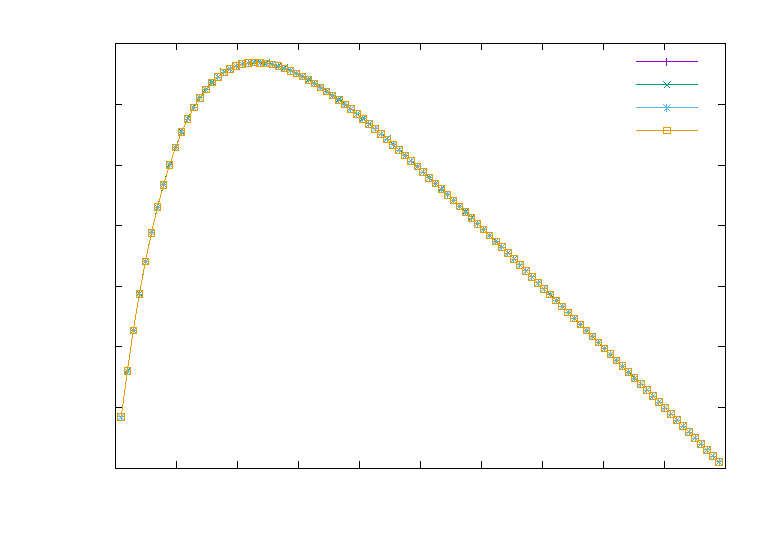
\includegraphics{solutionN100}}%
    \gplfronttext
  \end{picture}%
\endgroup
 }}%
    \caption{Results using the presented methods for $N=10$ (left) and $N=100$ (right)}
    \label{fig:n10}%
\end{figure}

\begin{figure}[t]
  \centering
  % GNUPLOT: LaTeX picture with Postscript
\begingroup
  \makeatletter
  \providecommand\color[2][]{%
    \GenericError{(gnuplot) \space\space\space\@spaces}{%
      Package color not loaded in conjunction with
      terminal option `colourtext'%
    }{See the gnuplot documentation for explanation.%
    }{Either use 'blacktext' in gnuplot or load the package
      color.sty in LaTeX.}%
    \renewcommand\color[2][]{}%
  }%
  \providecommand\includegraphics[2][]{%
    \GenericError{(gnuplot) \space\space\space\@spaces}{%
      Package graphicx or graphics not loaded%
    }{See the gnuplot documentation for explanation.%
    }{The gnuplot epslatex terminal needs graphicx.sty or graphics.sty.}%
    \renewcommand\includegraphics[2][]{}%
  }%
  \providecommand\rotatebox[2]{#2}%
  \@ifundefined{ifGPcolor}{%
    \newif\ifGPcolor
    \GPcolortrue
  }{}%
  \@ifundefined{ifGPblacktext}{%
    \newif\ifGPblacktext
    \GPblacktexttrue
  }{}%
  % define a \g@addto@macro without @ in the name:
  \let\gplgaddtomacro\g@addto@macro
  % define empty templates for all commands taking text:
  \gdef\gplbacktext{}%
  \gdef\gplfronttext{}%
  \makeatother
  \ifGPblacktext
    % no textcolor at all
    \def\colorrgb#1{}%
    \def\colorgray#1{}%
  \else
    % gray or color?
    \ifGPcolor
      \def\colorrgb#1{\color[rgb]{#1}}%
      \def\colorgray#1{\color[gray]{#1}}%
      \expandafter\def\csname LTw\endcsname{\color{white}}%
      \expandafter\def\csname LTb\endcsname{\color{black}}%
      \expandafter\def\csname LTa\endcsname{\color{black}}%
      \expandafter\def\csname LT0\endcsname{\color[rgb]{1,0,0}}%
      \expandafter\def\csname LT1\endcsname{\color[rgb]{0,1,0}}%
      \expandafter\def\csname LT2\endcsname{\color[rgb]{0,0,1}}%
      \expandafter\def\csname LT3\endcsname{\color[rgb]{1,0,1}}%
      \expandafter\def\csname LT4\endcsname{\color[rgb]{0,1,1}}%
      \expandafter\def\csname LT5\endcsname{\color[rgb]{1,1,0}}%
      \expandafter\def\csname LT6\endcsname{\color[rgb]{0,0,0}}%
      \expandafter\def\csname LT7\endcsname{\color[rgb]{1,0.3,0}}%
      \expandafter\def\csname LT8\endcsname{\color[rgb]{0.5,0.5,0.5}}%
    \else
      % gray
      \def\colorrgb#1{\color{black}}%
      \def\colorgray#1{\color[gray]{#1}}%
      \expandafter\def\csname LTw\endcsname{\color{white}}%
      \expandafter\def\csname LTb\endcsname{\color{black}}%
      \expandafter\def\csname LTa\endcsname{\color{black}}%
      \expandafter\def\csname LT0\endcsname{\color{black}}%
      \expandafter\def\csname LT1\endcsname{\color{black}}%
      \expandafter\def\csname LT2\endcsname{\color{black}}%
      \expandafter\def\csname LT3\endcsname{\color{black}}%
      \expandafter\def\csname LT4\endcsname{\color{black}}%
      \expandafter\def\csname LT5\endcsname{\color{black}}%
      \expandafter\def\csname LT6\endcsname{\color{black}}%
      \expandafter\def\csname LT7\endcsname{\color{black}}%
      \expandafter\def\csname LT8\endcsname{\color{black}}%
    \fi
  \fi
    \setlength{\unitlength}{0.0500bp}%
    \ifx\gptboxheight\undefined%
      \newlength{\gptboxheight}%
      \newlength{\gptboxwidth}%
      \newsavebox{\gptboxtext}%
    \fi%
    \setlength{\fboxrule}{0.5pt}%
    \setlength{\fboxsep}{1pt}%
\begin{picture}(7200.00,5040.00)%
    \gplgaddtomacro\gplbacktext{%
      \csname LTb\endcsname%
      \put(814,704){\makebox(0,0)[r]{\strut{}$-10$}}%
      \put(814,1156){\makebox(0,0)[r]{\strut{}$-9$}}%
      \put(814,1609){\makebox(0,0)[r]{\strut{}$-8$}}%
      \put(814,2061){\makebox(0,0)[r]{\strut{}$-7$}}%
      \put(814,2513){\makebox(0,0)[r]{\strut{}$-6$}}%
      \put(814,2966){\makebox(0,0)[r]{\strut{}$-5$}}%
      \put(814,3418){\makebox(0,0)[r]{\strut{}$-4$}}%
      \put(814,3870){\makebox(0,0)[r]{\strut{}$-3$}}%
      \put(814,4323){\makebox(0,0)[r]{\strut{}$-2$}}%
      \put(814,4775){\makebox(0,0)[r]{\strut{}$-1$}}%
      \put(946,484){\makebox(0,0){\strut{}$-6.5$}}%
      \put(1478,484){\makebox(0,0){\strut{}$-6$}}%
      \put(2011,484){\makebox(0,0){\strut{}$-5.5$}}%
      \put(2543,484){\makebox(0,0){\strut{}$-5$}}%
      \put(3076,484){\makebox(0,0){\strut{}$-4.5$}}%
      \put(3608,484){\makebox(0,0){\strut{}$-4$}}%
      \put(4141,484){\makebox(0,0){\strut{}$-3.5$}}%
      \put(4673,484){\makebox(0,0){\strut{}$-3$}}%
      \put(5206,484){\makebox(0,0){\strut{}$-2.5$}}%
      \put(5738,484){\makebox(0,0){\strut{}$-2$}}%
      \put(6271,484){\makebox(0,0){\strut{}$-1.5$}}%
      \put(6803,484){\makebox(0,0){\strut{}$-1$}}%
    }%
    \gplgaddtomacro\gplfronttext{%
      \csname LTb\endcsname%
      \put(176,2739){\rotatebox{-270}{\makebox(0,0){\strut{}Max Error}}}%
      \put(3874,154){\makebox(0,0){\strut{}$log_{10}(h)$}}%
      \csname LTb\endcsname%
      \put(5816,4602){\makebox(0,0)[r]{\strut{}Max Relative Error}}%
    }%
    \gplbacktext
    \put(0,0){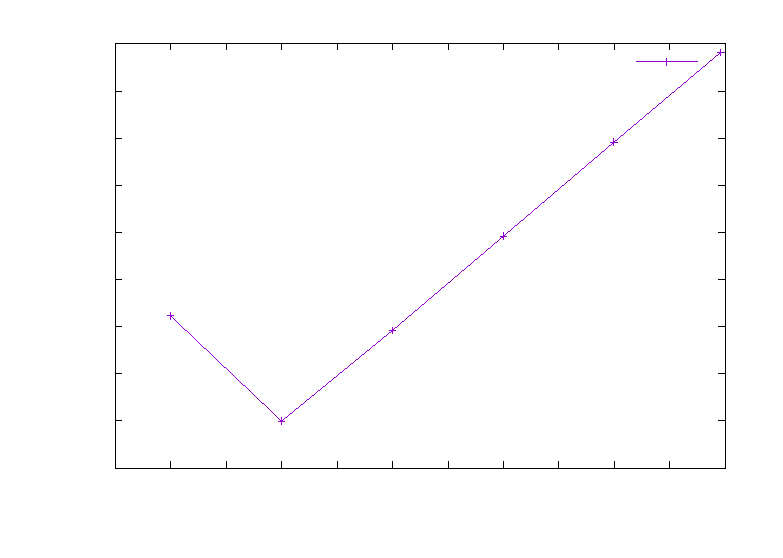
\includegraphics{error}}%
    \gplfronttext
  \end{picture}%
\endgroup

  \caption{Maximum relative error scaling with relative grid spacing }
  \label{fig:error}
\end{figure}
Another bottleneck found was in the case of the LU factorization method. By construction, the method requires a full matrix to be stored in memory unless the algorithm is modified in some fashion to accomadate sparse matrix storage, and thus the memory requirements become prohibitively large for grid sizes above $N=1000$. 
\subsection{Efficiency}
In the previous section it was shown that all methods are sufficiently accurate for modest grid sizes, thus we now investigate the corresponding computational times in \ref{table:time}. The specialized TDMA method does not improve significantly on the computational time of the general algorithm until the grid size surpasses $N=100$ while the LU-decomposition method remains significantly slower for all grids.  
\begin{table}[t]
\centering
\begin{tabular}{|c|c|c|c|}
	\hline
	N & TDMA & General & LU \\\hline 
	10 & $3.0\times10^{-6} $& $3.0\times10^{-6}$ & $2.0\times10^{-3}$\\
	100 & $5.1\times10^{-6} $& $6.5\times10^{-6}$ & $0.5\times10^{-3} $\\
	1000 & $3.5\times10^{-5}$ & $6.1\times10^{-5}$ & $5.7\times10^{-2}$\\
	10000 & $2.3\times10^{-4}$ & $1.2\times10^{-5}$ & 21.8\\\hline
\end{tabular}
  \caption{Computational times for varying grid size and algorithm}
	\label{table:time}
\end{table}

\section{Conclusion}
The comparisons shown in this work outline the trade-offs when it comes to choosing numerical algorithms for scientific computing. Gaussian elimination while general, may not be the best choice if a speed alone is of importance in solving the 1D poisson equation. While the LU decomposition method is both slow and memory intensive, it hold the distinct advantage of being completely general and portable. The advantage of an algorithm that can be ported over to another problem trivially is potentially very useful, especially if this leads to faster development and deployment of the code. The addition of human hours spent developing and testing is an important factor when choosing an algorithm to implement given a specific outcome desired. Additionally we have seen the vast improvements possible when refining an algorithm to a problem specific form as in the TDMA method. It is also interesting to note how applicable this trade-off of algorithm generality vs efficiency is to the debate over programming languages for implementation. Generally, an object-oriented programming language can significantly streamline the process of adapting an algorithm to a new problem, at the expense of computational time with respect to a non object oriented language such as FORTRAN.

\bibliographystyle{unsrt}
\bibliography{refs}
\end{document}